%% BioMed_Central_Tex_Template_v1.06
%%                                      %
%  bmc_article.tex            ver: 1.06 %
%                                       %

%%IMPORTANT: do not delete the first line of this template
%%It must be present to enable the BMC Submission system to
%%recognise this template!!

%%%%%%%%%%%%%%%%%%%%%%%%%%%%%%%%%%%%%%%%%
%%                                     %%
%%  LaTeX template for BioMed Central  %%
%%     journal article submissions     %%
%%                                     %%
%%          <8 June 2012>              %%
%%                                     %%
%%                                     %%
%%%%%%%%%%%%%%%%%%%%%%%%%%%%%%%%%%%%%%%%%


%%%%%%%%%%%%%%%%%%%%%%%%%%%%%%%%%%%%%%%%%%%%%%%%%%%%%%%%%%%%%%%%%%%%%
%%                                                                 %%
%% For instructions on how to fill out this Tex template           %%
%% document please refer to Readme.html and the instructions for   %%
%% authors page on the biomed central website                      %%
%% http://www.biomedcentral.com/info/authors/                      %%
%%                                                                 %%
%% Please do not use \input{...} to include other tex files.       %%
%% Submit your LaTeX manuscript as one .tex document.              %%
%%                                                                 %%
%% All additional figures and files should be attached             %%
%% separately and not embedded in the \TeX\ document itself.       %%
%%                                                                 %%
%% BioMed Central currently use the MikTex distribution of         %%
%% TeX for Windows) of TeX and LaTeX.  This is available from      %%
%% http://www.miktex.org                                           %%
%%                                                                 %%
%%%%%%%%%%%%%%%%%%%%%%%%%%%%%%%%%%%%%%%%%%%%%%%%%%%%%%%%%%%%%%%%%%%%%

%%% additional documentclass options:
%  [doublespacing]
%  [linenumbers]   - put the line numbers on margins

%%% loading packages, author definitions

%\documentclass[twocolumn]{bmcart}% uncomment this for twocolumn layout and comment line below
\documentclass{bmcart}
%  Recompile
%2


%%% Load packages
\usepackage{amsthm,amsmath}
\RequirePackage{natbib}
\usepackage{natbib}
\usepackage{graphicx}
\usepackage{subcaption}
\RequirePackage[authoryear]{natbib}% uncomment this for author-year bibliography
%\RequirePackage{hyperref}
\usepackage[utf8]{inputenc} %unicode support
%\usepackage[applemac]{inputenc} %applemac support if unicode package fails
%\usepackage[latin1]{inputenc} %UNIX support if unicode package fails
%\usepackage{natbib}

%%%%%%%%%%%%%%%%%%%%%%%%%%%%%%%%%%%%%%%%%%%%%%%%%
%%                                             %%
%%  If you wish to display your graphics for   %%
%%  your own use using includegraphic or       %%
%%  includegraphics, then comment out the      %%
%%  following two lines of code.               %%
%%  NB: These line *must* be included when     %%
%%  submitting to BMC.                         %%
%%  All figure files must be submitted as      %%
%%  separate graphics through the BMC          %%
%%  submission process, not included in the    %%
%%  submitted article.                         %%
%%                                             %%
%%%%%%%%%%%%%%%%%%%%%%%%%%%%%%%%%%%%%%%%%%%%%%%%%

%\def\includegraphic{}
%\def\includegraphics{}

%%% Put your definitions there:
\startlocaldefs
\endlocaldefs


%%% Begin ...
\begin{document}


%%% Start of article front matter
\begin{frontmatter}

\begin{fmbox}
\dochead{Research}

%%%%%%%%%%%%%%%%%%%%%%%%%%%%%%%%%%%%%%%%%%%%%%
%%                                          %%
%% Enter the title of your article here     %%
%%                                          %%
%%%%%%%%%%%%%%%%%%%%%%%%%%%%%%%%%%%%%%%%%%%%%%

\title{Prevalence and the variance of state occupancy time}

%%%%%%%%%%%%%%%%%%%%%%%%%%%%%%%%%%%%%%%%%%%%%%
%%                                          %%
%% Enter the authors here                   %%
%%                                          %%
%% Specify information, if available,       %%
%% in the form:                             %%
%%   <key>={<id1>,<id2>}                    %%
%%   <key>=                                 %%
%% Comment or delete the keys which are     %%
%% not used. Repeat \author command as much %%
%% as required.                             %%
%%                                          %%
%%%%%%%%%%%%%%%%%%%%%%%%%%%%%%%%%%%%%%%%%%%%%%

\author[
   addressref={aff1},                   % id's of addresses, e.g. {aff1,aff2}
   corref={aff1},                       % id of corresponding address, if any
   noteref={n1},                        % id's of article notes, if any
   email={riffe@demogr.mpg.de}   % email address
]{\inits{TR}\fnm{Tim} \snm{Riffe}}
%\author[
%   addressref={aff1,aff2},
%   email={john.RS.Smith@cambridge.co.uk}
%]{\inits{JRS}\fnm{John RS} \snm{Smith}}

%%%%%%%%%%%%%%%%%%%%%%%%%%%%%%%%%%%%%%%%%%%%%%
%%                                          %%
%% Enter the authors' addresses here        %%
%%                                          %%
%% Repeat \address commands as much as      %%
%% required.                                %%
%%                                          %%
%%%%%%%%%%%%%%%%%%%%%%%%%%%%%%%%%%%%%%%%%%%%%%

\address[id=aff1]{%                           % unique id
  \orgname{Max-Planck-Institute for Demographic Research}, % university, etc
  \street{Konrad-Zuse-Str. 1},                     %
  \postcode{18057}                                % post or zip code
  \city{Rostock},                              % city
  \cny{Germany}                                    % country
}

%%%%%%%%%%%%%%%%%%%%%%%%%%%%%%%%%%%%%%%%%%%%%%
%%                                          %%
%% Enter short notes here                   %%
%%                                          %%
%% Short notes will be after addresses      %%
%% on first page.                           %%
%%                                          %%
%%%%%%%%%%%%%%%%%%%%%%%%%%%%%%%%%%%%%%%%%%%%%%

\begin{artnotes}
\note{This manuscript is in its early stages}     % note to the article
\note[id=n1]{~} % note, connected to author
\end{artnotes}

\end{fmbox}% comment this for two column layout

%%%%%%%%%%%%%%%%%%%%%%%%%%%%%%%%%%%%%%%%%%%%%%
%%                                          %%
%% The Abstract begins here                 %%
%%                                          %%
%% Please refer to the Instructions for     %%
%% authors on http://www.biomedcentral.com  %%
%% and include the section headings         %%
%% accordingly for your article type.       %%
%%                                          %%
%%%%%%%%%%%%%%%%%%%%%%%%%%%%%%%%%%%%%%%%%%%%%%

\begin{abstractbox}

\begin{abstract} % abstract
\parttitle{Background} 
Markov reward methods have been proposed to calculate the variance of state occupancy time based on age-structured prevalence and survivorship.
\parttitle{Objectives} I aim to clarify the assumptions of this approach, give bounds to its reasonableness, and suggest improvements.
\parttitle{Methods} I calculate results for extreme cases to provide bounds, I simulate the variance under simple assumptions, and simulate a more natural inter-individual state distribution.
\parttitle{Results} I show that state occupancy variance for Sullivan-style inputs is not identified, and I show where previously proposed methods fall with respect to reasonable bounds, randomly generated variances, and my own opinion about what a reasonable inter-individual state distribution might look like.
\parttitle{Conclusions} 
The variance of state occupancy time is only identified if a) state life trajectories are directly observed or b) a process model, such as an incidence-based Markov model, is specified. Sullivan-calculations of life expectancy do not imply a single variance, and are therefore insufficient to make statements on inter-individual disparities in state occupancies.
\end{abstract}

%%%%%%%%%%%%%%%%%%%%%%%%%%%%%%%%%%%%%%%%%%%%%%
%%                                          %%
%% The keywords begin here                  %%
%%                                          %%
%% Put each keyword in separate \kwd{}.     %%
%%                                          %%
%%%%%%%%%%%%%%%%%%%%%%%%%%%%%%%%%%%%%%%%%%%%%%

\begin{keyword}
\kwd{Healthy life expectancy}
\kwd{Sullivan method}
\kwd{Healthy life variance}
\end{keyword}

% MSC classifications codes, if any
%\begin{keyword}[class=AMS]
%\kwd[Primary ]{}
%\kwd{}
%\kwd[; secondary ]{}
%\end{keyword}

\end{abstractbox}
%

%\end{fmbox}% uncomment this for twcolumn layout

\end{frontmatter}

%%%%%%%%%%%%%%%%%%%%%%%%%%%%%%%%%%%%%%%%%%%%%%
%%                                          %%
%% The Main Body begins here                %%
%%                                          %%
%% Please refer to the instructions for     %%
%% authors on:                              %%
%% http://www.biomedcentral.com/info/authors%%
%% and include the section headings         %%
%% accordingly for your article type.       %%
%%                                          %%
%% See the Results and Discussion section   %%
%% for details on how to create sub-sections%%
%%                                          %%
%% use \cite{...} to cite references        %%
%%  \cite{koon} and                         %%
%%  \cite{oreg,khar,zvai,xjon,schn,pond}    %%
%%  \nocite{smith,marg,hunn,advi,koha,mouse}%%
%%                                          %%
%%%%%%%%%%%%%%%%%%%%%%%%%%%%%%%%%%%%%%%%%%%%%%

\section*{Introduction}
Healthy inquality is usually measured between populations by comparing life expectancies, health expectancies, or poor health expectancies. Within populations there is also inquality in health outcomes, either due to violations of the assumption of homogeneity of risk sets or due to random variation between people otherwise subject to the same risk.

bla bla I'll end up proposing some alternative variance calcs for Sullivan situations, but also that these are always hypothetical and that in fact the variance is not determined, and has a rather wide potential range of values depending on actual life trajectories.

\section*{Sullivan in continuous time}
Let's begin with some familiar notation, $\ell(x)$ denotes lifetable survivorship, with an arbitrary radix, or starting population. If $\ell(0) = 1$ then $\ell(x)$ can be interpreted as a probability of surviving from birth until age $x$. $\pi(x)$ is the prevalence of a given condition (healthiness or unhealthiness, disability) at age $x$, and it falls in the range $[0,1]$, giving it a probability interpretation. The commonly used Sullivan method \citep{sullivan1971single} of calculating healthy life expectancy, $e^H(x)$ is to integrate the product of these two functions.
%
\begin{equation}
\label{eq:sull}
e^H(x) = \frac{1}{\ell(x)} \int_x^\omega \ell(t)\pi(t) \mathrm{d}t
\end{equation}
%

Replace $\pi$ with its complement to arrive at the complementary expectancy, $e^U(x)$, such that overall life expectancy for this age is $e(x) = e^U(x) + e^H(x)$, a rudimentary composition.

\section*{Two assumptions}
If we would like to know something about the variance of state occupancy in a Sullivan setup, then we must make some assumptions about how the state is distributed over individuals. The Sullivan method does not state which between-individual state distribution underlies prevalence in a given age. If $\pi(x) = 0.5$, shall we assign each individual age $x$ a value of 0.5 a so-called \emph{fixed reward}, or shall we assign half of them a value of 1, and the other half a value of 0, a \emph{Bernoulli reward} \citep{caswell2018matrix}? Or something else entirely? There are infinitely many ways to distribute state $\pi$ among individuals in age $x$ such that the value $\pi(x)$ is maintained. By extension, the inter-individual distribution of total time spent in state $\pi$ is also infinitely variable, which implies that the variance and other moments of implied state occupancy are not uniquely identified. 

Expressing the lifetable as a Markov chain with \emph{rewards} defined as prevalence gives a unique definition for the variance of state occupancy for each of the above assumptions, but it is unclear to me how well-supported these are. Many other reward types are discussed by Caswell \& Zarulli \cite{caswell2018matrix}, and I do not discuss these, nor do I treat the case of multistate populations. Even so, the conclusions reached here will generalize to the case of multistate populations.

%We will use two shorthand and equivalent forms to calculate variance, depending on the situation. First the mean of the squared residuals:
%\begin{equation}
%Var(X) = \mathbb{E}\left[(X-\mathbb{E}[X])^2 \right] \quad \mathrm{,}
%\end{equation}
%where in practice the outer expectation is taken as the sum of the squared residuals duly weighted by their respective probabilities of ocurring. The second is

\subsection*{Bernoulli rewards}
I'll first give my own lifetable deconstruction of the matrix algebra approach given to Bernoulli state variance in \cite{caswell2018matrix}. Then $e^H(x)$ is defined per \eqref{eq:sull}, and it is the first moment of state occupancy, which we can denote $\eta^{(1)}$, where the superscript in parentheses denotes the moment number and is not a power. We continue to calculate the second moment of state occupancy, $\eta^{(2)}$ as:
\begin{equation}
\label{eq:bern2}
\eta^{(2)}_x = \frac{1}{\ell_x} \sum_{t=x}^\omega \ell_t\left[\pi_t + 2(1-q_t)\pi_t\eta^{(1)}_t\right] \quad \mathrm{,}
\end{equation}
where $q_x$ is the probability of death in the interval and $\omega$ is the highest age of death. Here notation omits intervals, but we assume to be working in discrete bins, where death and transition changes only happen in the moment of interval steps, implying a stepped survival curve and discrete life trajectories. We also assume that the same prevalence applies to each length-of-life bin, ergo that all other unomodelled population strata have the same prevalence. Then the variance is determined, and it can be calculated as:
\begin{equation}
\label{eq:var2}
Var_x = \eta^{(2)}_x - (\eta^{(1)}_x)^2
\end{equation}

I highlight two assumptions behind this expression: 1) mortality is independent of whether one is in the prevalent state, and 2) the same Bernoulli prevalence extends to any further stratification of the members in a given age class, $x$.

\subsection*{Fixed rewards}
If instead of assuming that prevalence is partioned in a binary fashion, and each individual experiences $\pi_x$ fraction of the year in the state, then equation \eqref{eq:bern2} becomes
\begin{equation}
\eta^{(2)}_x = \frac{1}{\ell_x} \sum_{t=x}^\omega \ell_t\left[\pi_t^2 + 2(1-q_t)\pi_t\eta^{(1)}_t\right] \quad \mathrm{,}
\end{equation}
and \eqref{eq:var2} is the same.

\subsection{Illustrations of Bernoulli and fixed prevalence}
\begin{figure}
    \centering
    \begin{subfigure}[b]{0.3\textwidth}
        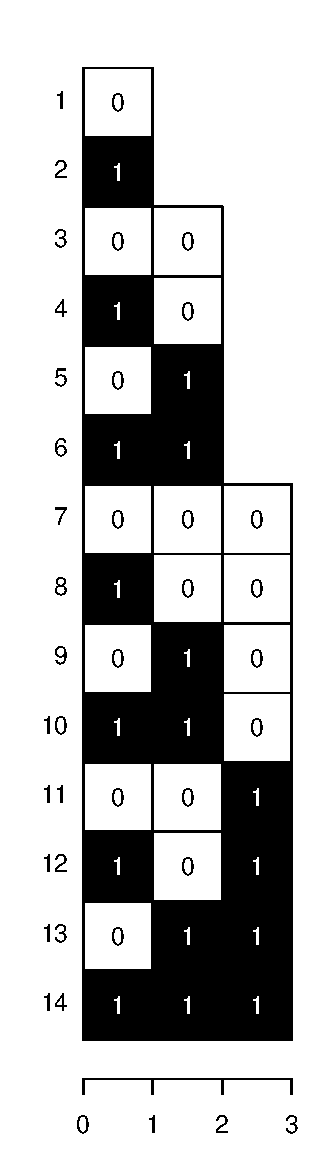
\includegraphics[width=\textwidth]{Figures/BernTraj.pdf}
        \caption{The binary 2-state trajectory space.}
        \label{fig:b1}
    \end{subfigure}
    ~ 
    \begin{subfigure}[b]{0.3\textwidth}
        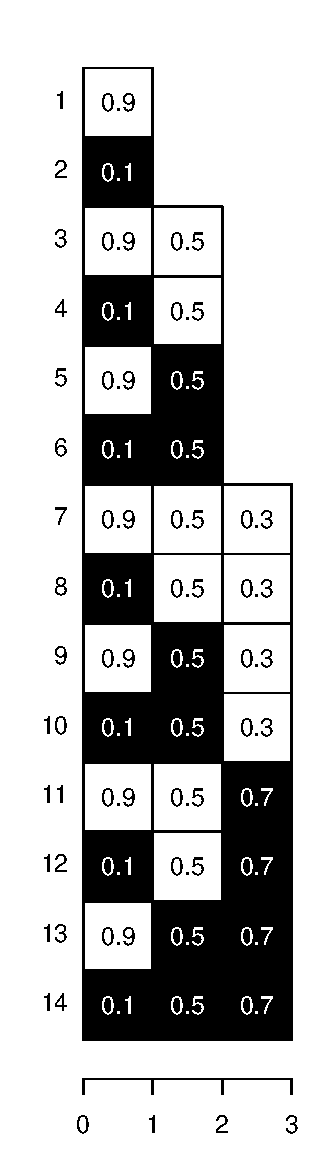
\includegraphics[width=\textwidth]{Figures/BernTrajProbs.pdf}
        \caption{With Bernoulli prevalence cell probabilities.}
        \label{fig:b2}
    \end{subfigure}
    
     \begin{subfigure}[b]{0.3\textwidth}
        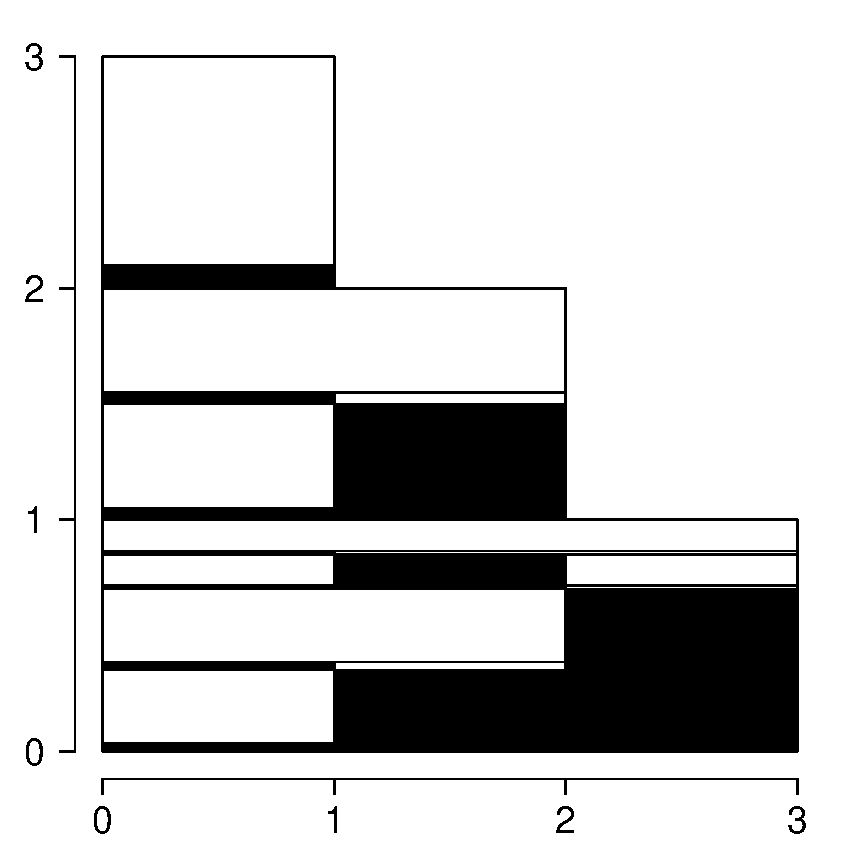
\includegraphics[width=\textwidth]{Figures/BernCondTrajProbs.pdf}
        \caption{With trajectories Bernoulli weighted, conditional on length of life.}
        \label{fig:b3}
    \end{subfigure}
    ~ 
    \begin{subfigure}[b]{0.3\textwidth}
        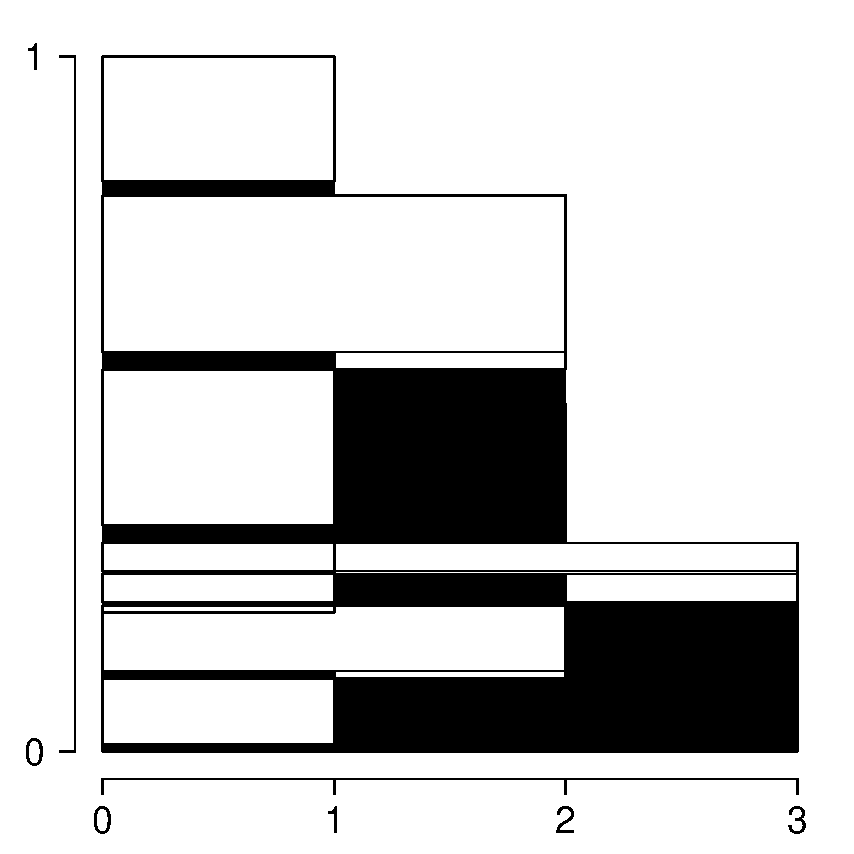
\includegraphics[width=\textwidth]{Figures/BernTrajProbsWeighted}
        \caption{With trajectories Bernoulli and lifetable weighted.}
        \label{fig:b4}
    \end{subfigure}
    \caption{A depiction of the Bernoulli life trajectories implied by the prevalence and lifetable of Tab.~\ref{}}\label{fig:bernexplain}
\end{figure}

%\nocite{oreg,schn,pond,smith,marg,hunn,advi,koha,mouse}

%%%%%%%%%%%%%%%%%%%%%%%%%%%%%%%%%%%%%%%%%%%%%%
%%                                          %%
%% Backmatter begins here                   %%
%%                                          %%
%%%%%%%%%%%%%%%%%%%%%%%%%%%%%%%%%%%%%%%%%%%%%%

\begin{backmatter}

\section*{Competing interests}
  The authors declare that they have no competing interests.

\section*{Author's contributions}
    TR did everything.

\section*{Acknowledgements}
  Thanks to Douglas Wolf and Jennifer Karas Montez for posing a question that led to this work, and to Hal Caswell and Virginia Zarulli for the groundwork on which this is based and for fielding inquiries.
%%%%%%%%%%%%%%%%%%%%%%%%%%%%%%%%%%%%%%%%%%%%%%%%%%%%%%%%%%%%%
%%                  The Bibliography                       %%
%%                                                         %%
%%  Bmc_mathpys.bst  will be used to                       %%
%%  create a .BBL file for submission.                     %%
%%  After submission of the .TEX file,                     %%
%%  you will be prompted to submit your .BBL file.         %%
%%                                                         %%
%%                                                         %%
%%  Note that the displayed Bibliography will not          %%
%%  necessarily be rendered by Latex exactly as specified  %%
%%  in the online Instructions for Authors.                %%
%%                                                         %%
%%%%%%%%%%%%%%%%%%%%%%%%%%%%%%%%%%%%%%%%%%%%%%%%%%%%%%%%%%%%%

% if your bibliography is in bibtex format, use those commands:
\bibliographystyle{bmc-mathphys} % Style BST file (bmc-mathphys, vancouver, spbasic).
\bibliography{references}      % Bibliography file (usually '*.bib' )
% for author-year bibliography (bmc-mathphys or spbasic)
% a) write to bib file (bmc-mathphys only)
% @settings{label, options="nameyear"}
% b) uncomment next line
%\nocite{label}

% or include bibliography directly:
% \begin{thebibliography}
% \bibitem{b1}
% \end{thebibliography}

%%%%%%%%%%%%%%%%%%%%%%%%%%%%%%%%%%%
%%                               %%
%% Figures                       %%
%%                               %%
%% NB: this is for captions and  %%
%% Titles. All graphics must be  %%
%% submitted separately and NOT  %%
%% included in the Tex document  %%
%%                               %%
%%%%%%%%%%%%%%%%%%%%%%%%%%%%%%%%%%%

%%
%% Do not use \listoffigures as most will included as separate files

%\section*{Figures}
%  \begin{figure}[h!]
%  \caption{\csentence{Sample figure title.}
%      A short description of the figure content
%      should go here.}
%      \end{figure}

%\begin{figure}[h!]
%  \caption{\csentence{Sample figure title.}
%      Figure legend text.}
%      \end{figure}

%%%%%%%%%%%%%%%%%%%%%%%%%%%%%%%%%%%
%%                               %%
%% Tables                        %%
%%                               %%
%%%%%%%%%%%%%%%%%%%%%%%%%%%%%%%%%%%

%% Use of \listoftables is discouraged.
%%
%\section*{Tables}
%\begin{table}[h!]
%\caption{Sample table title. This is where the description of the table should
% go.}
%      \begin{tabular}{cccc}
%        \hline
%           & B1  &B2   & B3\\ \hline
%        A1 & 0.1 & 0.2 & 0.3\\
%        A2 & ... & ..  & .\\
%        A3 & ..  & .   & .\\ \hline
%      \end{tabular}
%\end{table}

%%%%%%%%%%%%%%%%%%%%%%%%%%%%%%%%%%%
%%                               %%
%% Additional Files              %%
%%                               %%
%%%%%%%%%%%%%%%%%%%%%%%%%%%%%%%%%%%

\section*{Additional Files}
  \subsection*{Additional file 1 --- Sample additional file title}
    Additional file descriptions text (including details of how to
    view the file, if it is in a non-standard format or the file extension).  This might
    refer to a multi-page table or a figure.

  \subsection*{Additional file 2 --- Sample additional file title}
    Additional file descriptions text.


\end{backmatter}
\end{document}
